\begin{frame}
\frametitle{Non-word Error Detection Data}
\centering
\begin{itemize}
\item {\textasciitilde}120k positive examples (Aspell English dictionary)
\item {\textasciitilde}360k non-words (transpose, insert, substitute, or delete) \\
\item Imbalanced target distribution $\implies$ needed to scale the value of loss function for each minibatch.
\item Assume \textit{closed} universe of words, so \textit{test} on \textit{training} set. 
\end{itemize}
\begin{tabular}{lc}
\multicolumn{1}{c}{\textsc{Input}} & \textsc{Target} \\
\hline
{\string^}acclimate\$ & 1 \\
{\string^}aclcimate\$ & 0 \\
{\string^}wellsprings\$ & 1 \\
{\string^}wellsprigns\$ & 0 \\
{\string^}mistype\$ & 1 \\
{\string^}mitsype\$ & 0 \\
\end{tabular}
\end{frame}

\begin{frame}
\centering
\begin{tabular}{lcccc}
\textsc{Operation} & \textsc{Precision} & \textsc{Recall} & \textsc{F1} & \textsc{N} \\
\hline
Transpose & \textbf{0.996} & \textbf{0.999} & \textbf{0.998} & 475,535 \\
Insert &  0.994 & \textbf{0.999} & 0.997 & 479,092 \\
Substitute & 0.976 & 0.997 & 0.986 & 478,988 \\
Delete & 0.905 & 0.989 & 0.945 & 473,786\\
\end{tabular}
\end{frame}

%\begin{frame}
%\input figures/chapter03/confusion-matrices.tex
%\end{frame}

\begin{frame}
\centering
\input figures/chapter03/confusion-matrix.tex
\end{frame}

\begin{frame}
\centering
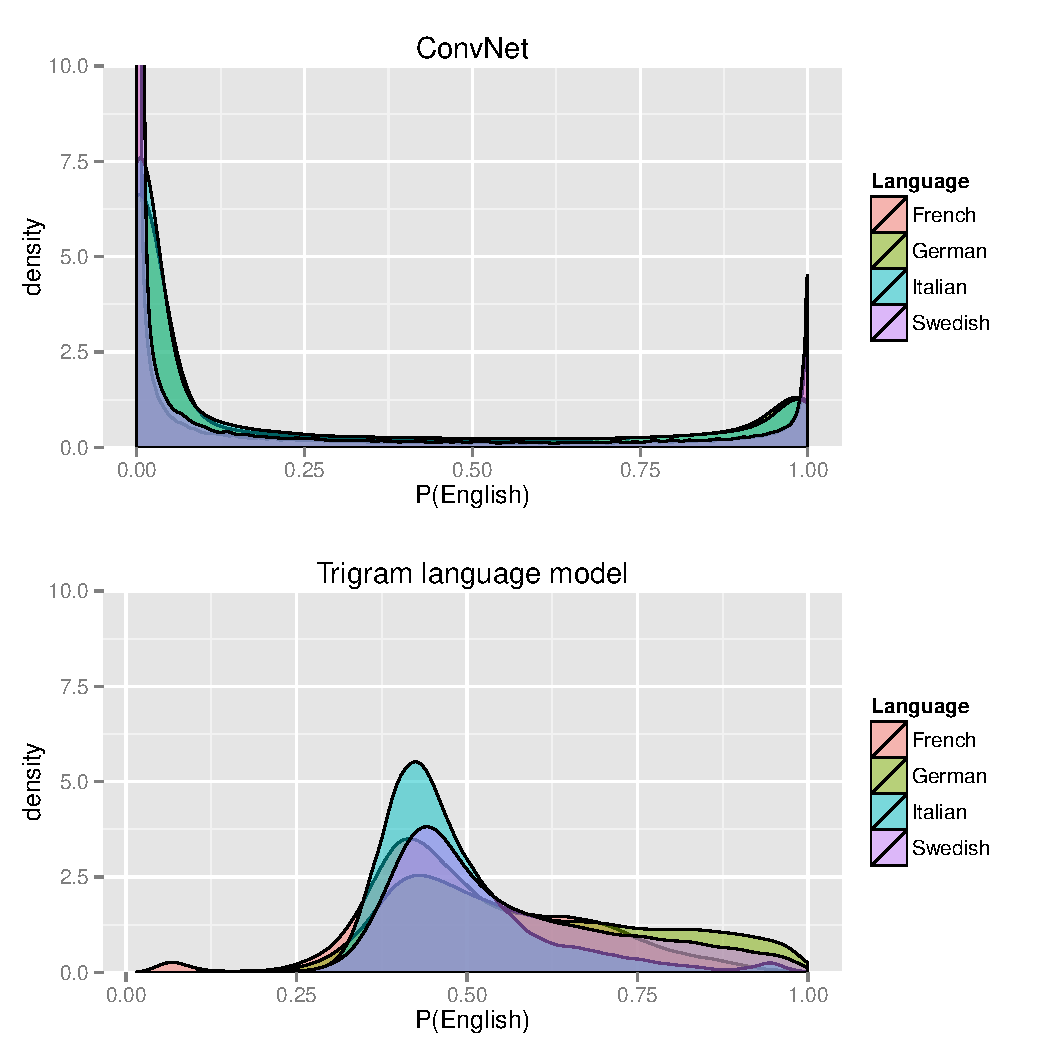
\includegraphics[height=0.99\textheight]{figures/chapter03/languages-convnet-vs-lm}
\end{frame}

\begin{frame}
\centering
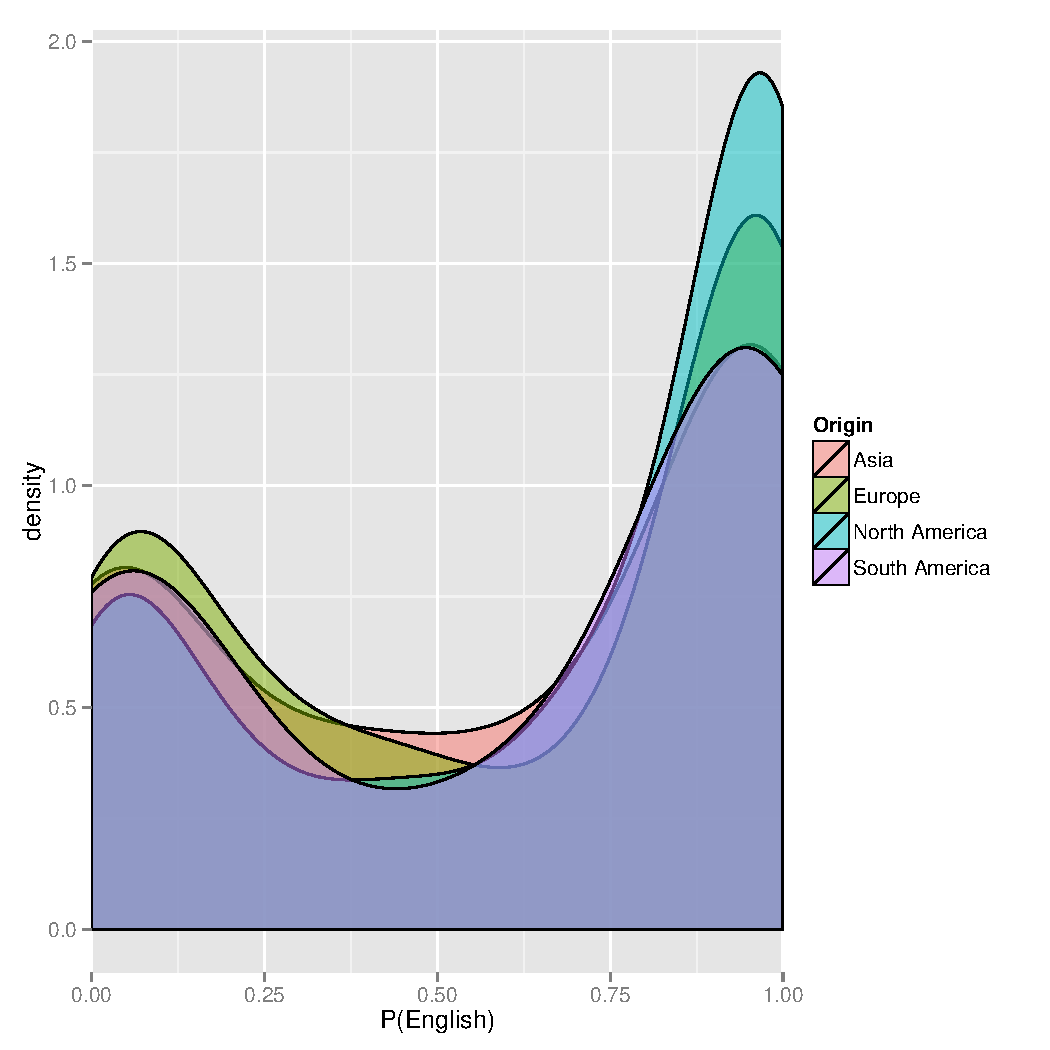
\includegraphics[height=0.99\textheight]{figures/chapter03/brands-convnet}
\end{frame}
